\ifx \allfiles \undefined
\documentclass[12pt,a4paper,oneside]{report}

%% === CJK 套件 ===
\usepackage{CJKutf8,CJKnumb}                 % 中文套件
%% === AMS 標準套件 ===
\usepackage{amsmath,amsfonts,amssymb,amsthm} % 數學符號
%% === ===
\usepackage{algorithm}
\usepackage{listings}                        % 程式碼
%% === TikZ 套件 ===
\usepackage{tikz,tkz-graph,tkz-berge}        % 繪圖
\usepackage{multicol}
%% == ==
\usepackage[unicode]{hyperref}
\usepackage{xcolor}
\hypersetup{
    colorlinks,
    linkcolor={blue!100!black},
    citecolor={blue!75!black},
    urlcolor={blue!50!black}
}
%% == 調整設定 ==
\usepackage{enumitem}                           % 修改 enumerate, item
\usepackage{bbding}
\usepackage{titletoc,titlesec,imakeidx}
%% == ==
\usepackage{newfloat}
\usepackage{caption,subcaption}
\usepackage{xkeyval,xargs}
\usepackage{ulem}
\usepackage{import}

%% === 設定 C++ 格式 ===
\lstset{%
  language=C++,             % 設定語言
  %% === 空白, tab 相關 ===
  tabsize=2,                % 設定 tab = 多少空白
  %showspaces=true,          % 設定是否標示空白
  %showtabs=true,            % 設定是否標示 tab
  %tab=\rightarrowfill,      % 設定 tab 樣式
  %% === 行數相關 ===
  numbers=left,             % 行數標示位置
  stepnumber=1,             % 每隔幾行標示行數
  numberstyle=\tiny,
  %breaklines=true,          % 設定斷行
  %% === 顏色設定 ===
  basicstyle=\ttfamily,
  keywordstyle=\color{blue}\ttfamily,
  stringstyle=\color{red!50!brown}\ttfamily,
  commentstyle=\color{green!50!black}\ttfamily,
  %identifierstyle=\color{black}\ttfamily,
  emphstyle=\color{purple}\ttfamily,
  extendedchars=false,
  texcl=true,
  moredelim=[l][\color{magenta}]{\#},
  captionpos=b,
  %% === 其他 ===
  %frame=single
}

% ===============================================
%
%  設定頁面格式
%
% ===============================================
%% === 設定頁面格式 ===
%\hoffset         = 10pt                      % 水平位移,預設為 0pt
\voffset         = -15pt                     % 垂直位移,預設為 0pt
\oddsidemargin   = 0pt                       % 預設為 31pt
%\topmargin       = 20pt                      % 預設為 20pt
%\headheight      = 12pt                      % header 的高度,預設為 12pt
%\headsep         = 25pt                      % header 和 body 的距離,預設為 25pt
\textheight      = 620pt                     % body 內文部分的高度,預設為 592pt
\textwidth       = 450pt                     % body 內文部分的寬度,預設為 390pt
%\marginparsep    = 10pt                      % margin note 和 body 的距離,預設為 10pt
%\marginparwidth  = 35pt                      % margin note 的寬度,預設為 35pt
%\footskip        = 30pt                      % footer 高度 + footer 和 body 的距離,預設為 30pt

%% ==  ==
\DeclareFloatingEnvironment[fileext=frm,placement={!ht},name=Frame]{code}
\captionsetup[code]{labelfont=bf}

\makeindex

\linespread{1.14}

\begin{document}
\begin{CJK}{UTF8}{bkai}

\subimport{./config/}{docsetting.tex}
\setcounter{chapter}{1}

\fi

\tikzset{bit block/.style={
	draw,
	rectangle,
	minimum height=\myht*\sz,
	minimum width=\mywd*\sz
}}
\tikzset{line arrow/.style={
	thick,
	latex-latex,
	-triangle 45
}}

\chapter{程式架構解析}

\paragraph{}這一節主要延續上一節的思維,但著重在了解程式如何執行,利用這些知識順利寫出\textbf{架構簡潔}、\textbf{容易除錯}程式。因此在這一節練習題較少,大多是\textbf{重要的觀念}。

\section*{本章目標}

\begin{itemize}
\item 了解記憶體與指標的概念
\item 利用選擇結構和迴圈結構
\item 物件導向的觀念
\end{itemize}

\section{位址與指標}

\subsection{溢位現象}

\paragraph{}以下程式碼會發生什麼現象?
\begin{code}[h!]
\centering
\begin{tabular}{c}
\begin{lstlisting}
int x = 2147483647;
cout << x + 1 << endl;
\end{lstlisting}
\end{tabular}
\caption{產生溢位的程式碼}
\label{program:struct:code:overflow}
\end{code}

\paragraph{}上一節提到 \lstinline!int! 的定義為「至少 2 個位元組」,若讀者的 \lstinline!int! 也是 4 個位元組的話,那麼就會得到 \lstinline!-2147483648!!這種現象我們稱為\index{溢位}{\textbf{溢位現象 (Overflow)}}。我們從二進位下看這段程式,會比較了解:

\begin{table}[h!]
\centering
\begin{tabular}{|c|c|c|c|}
\hline
$01111111$ & $11111111$ & $11111111$ & $11111111$\\
\hline
\end{tabular}
\caption{\lstinline!2147483647!}
\label{program:struct:table:binary:2147483647}
\end{table}

\paragraph{}表 \ref{program:struct:table:binary:2147483647} 表示 \lstinline!2147483647! 在 \texttt{C++} 當中如何儲存,讀者可以驗證 $2147483647=2^{31}-1$。若我們此時對 \lstinline!2147483647! 加 \lstinline!1!,就會得到下面的結果:

\begin{table}[h!]
\centering
\begin{tabular}{|c|c|c|c|}
\hline
${\color{red}1}0000000$ & $00000000$ & $00000000$ & $00000000$\\
\hline
\end{tabular}
\caption{\lstinline!2147483647 + 1!}
\end{table}

\paragraph{}用 \lstinline!int! 的儲存方法驗證,這個數字就是 \lstinline!-2147483648!,也就是 $-2^{32}$!為什麼會這樣子呢?
\paragraph{}大體上,表示資料的記憶體大小是\textbf{有限}的,那麼就會有以下兩種事情發生:
\begin{itemize}
\item 只能表示\textbf{有限多種}資料。例如:\lstinline!int! 通常是 4 個位元組,也就是 $4\times{8}=32$ 個位元,每個位元只能表示 \lstinline!0! 和 \lstinline!1! 兩種可能性,則最多只能表示 $2^{32}$ 種整數。這些可能性切一半,$2^{31}$ 個表示負整數,$2^{31}$ 表示非負整數,其中有一個 $0$,剩下 $2^{31}-1$ 個是正整數,因此 \lstinline!int! 的範圍就是介於 $-2^{31}$ 到 $2^{31}-1$。
\item \textbf{精確度}的限制。資料型態 \lstinline!double! 是以 \href{https://zh.wikipedia.org/wiki/IEEE_754}{IEEE 754} 為標準,有 8 個位元組,最多只能表示 $2^{64}$ 種小數。因為在標準中,以 53 個位元儲存尾數,故有 52 位有效數字,精確度為 $\log{2^{52}}\approx{15.95}$ 位十進位有效數字 (\lstinline!float! 則為 7 位)。
\end{itemize}

\begin{table}[h!]
\centering
\begin{tabular}{|c|c|c|c|}
\hline
\textbf{資料型態} & \textbf{位元組} & \textbf{通常下界} & \textbf{通常上界}\\
\hline\hline
\lstinline!char!      & 1 & $-128$        & $127$       \\
\hline
\lstinline!short!     & 2 & $-32768$      & $32767$     \\
\hline
\lstinline!int!       & 4 & $-2147483648$ & $2147483647$\\
\hline
\lstinline!long long! & 8 & $-9223372036854775808$ & $9223372036854775807$\\
\hline
\lstinline!float!     & 4 & $-3.40282\times{10^{38}}$ & $3.40282\times{10^{38}}$\\
\hline
\lstinline!double!    & 8 & $-1.79769\times{10^{308}}$ & $1.79769\times{10^{308}}$\\
\hline
\lstinline!unsigned char!      & 1 & $0$ & $255$\\
\hline
\lstinline!unsigned short!     & 2 & $0$ & $65535$\\
\hline
\lstinline!unsigned int!       & 4 & $0$ & $4294967295$\\
\hline
\lstinline!unsigned long long! & 8 & $0$ & $18446744073709551615$\\
\hline
\end{tabular}
\caption{資料型態上下界}
\label{program:struct:table:datatype:limit}
\end{table}

\paragraph{}表 \ref{program:struct:table:datatype:limit} 表示每一種資料型態常見的上下界範圍,其中 \lstinline!unsigned! 類型代表「\textbf{不帶負號}」,也就是說 \lstinline!unsigned! 系列會把所有符號拿去表示非負數。
\paragraph{}此外,需要注意的有幾點:
\begin{itemize}
\item \lstinline!int! 的上限是 \lstinline!2147483647!,用十六進位表示為 \lstinline!0x7FFFFFFF!
\item \lstinline!long long! 範圍大概是 $-9\times{10^{18}}$ 到 $9\times{10^{18}}$ 之間
\item \lstinline!double! 的範圍介於 $-{10}^{308}$ 至 ${10}^{308}$ 左右
\end{itemize}
\paragraph{}這些範圍可以在標頭檔 \index{標頭檔!climits}{\lstinline!<climits>!} 和 \index{標頭檔!cfloat}{\lstinline!<cfloat>!} 當中查詢到,實際範圍會依據不同計算機而有差異,查詢的方法自行 google,這裡不贅述。

\subsection{位址}

\subsubsection{記憶體}

\paragraph{}上一節提到\index{位元}{位元}和\index{位元組}{位元組}以及 \lstinline!sizeof! 等觀念,接下來要進入有關\index{記憶體}{\textbf{記憶體}}的部分。首先,我們常常提到的記憶體有分廣義和狹義,廣義的記憶體可以指稱所有儲存資料的設備,表 \ref{program:struct:table:hierarchical:memory} 列出計算機中常用的儲存設備:

\begin{table}[h!]
\centering
\begin{tabular}{|c|c|c|c|c|}
\hline
\textbf{種類}                                          & \textbf{原文} & \textbf{存取速度} & \textbf{容量} & \textbf{用途}                                              \\
\hline\hline
\color{blue}\textbf{暫存器} & Register & 1 CPU  週期 & 數百 Bytes 內 & \begin{tabular}[c]{@{}c@{}}CPU 內部暫存\\ 運算的資料\end{tabular}   \\
\hline
快取記憶體 & Cache & 數十 CPU 週期 & 數十 MB 內 & \begin{tabular}[c]{@{}c@{}}協調 CPU 和\\ 主記憶體的速度\end{tabular} \\
\hline
\color{red}\textbf{主記憶體} & Main Memory & 數百 CPU 週期 & 8 GB 左右 & \begin{tabular}[c]{@{}c@{}}執行程式、\\ 暫存資料等\end{tabular}      \\
\hline
\color{blue}\textbf{\begin{tabular}[c]{@{}c@{}}碟盤設備\\ (硬碟、光碟)\end{tabular}} & Disk Storage & 數百萬 CPU 周期 & 數 TB          & \begin{tabular}[c]{@{}c@{}}永久儲存\\ 程式、資料\end{tabular}       \\
\hline
\end{tabular}
\caption{廣義的記憶體,又稱為\textbf{記憶體階層} (2016 年資料)}
\label{program:struct:table:hierarchical:memory}
\end{table}

\paragraph{}狹義的記憶體就是\textbf{主記憶體},俗稱「\index{記憶體}{\textbf{記憶體}}」,程式在開始運行前,會將存在硬碟當中的程式資料移到記憶體當中,才會執行程式。

\subsubsection{位址概念}

\paragraph{}主記憶體可以看做是一條很長、連續的位元組,程式執行時,會佔據其中一個區塊,如圖 \ref{program:struct:fig:memory:and:program}:

\begin{figure}[h!]
\centering
\begin{tikzpicture}
\edef\mywd{2}
\draw (0,0) rectangle (13,\mywd);
\filldraw[black!40!white,draw=black] (0,0) rectangle (3,\mywd) node[black,pos=0.5] {作業系統};
\filldraw[black!30!white,draw=black] (3,0) rectangle (4,\mywd) node[black,pos=0.5] {程式};
\filldraw[black!30!white,draw=black] (5,0) rectangle (7,\mywd) node[black,pos=0.5] {程式};
\filldraw[black!30!white,draw=black] (7,0) rectangle (9,\mywd) node[black,pos=0.5] {程式};
\node at (-1,.5*\mywd) {記憶體};
\end{tikzpicture}
\caption{記憶體與程式}
\label{program:struct:fig:memory:and:program}
\end{figure}

\paragraph{}記憶體可以比作「\textbf{土地}」,一開始有一大片未經使用的土地,由作業系統和程式去分配用途 (當成 \lstinline!int!、\lstinline!double! 等)。為了方便管理記憶體,計算機會幫每個{\color{blue}\textbf{位元組}}標記「\textbf{地址}」,在此我們就稱為「\index{位址}{\color{red}\textbf{位址}}」。
\paragraph{}位元組是擁有地址的{\color{blue}\textbf{最小單位}},單個位元並沒有位址。

\subsubsection{取址運算子}

\paragraph{}位址是一個數字,通常以十六進位表示,如果要知道一個變數的位址,可以使用\index{取址運算子}{取址運算子} \lstinline!&!,例如程式碼 \ref{program:struct:code:address}:

\begin{code}[h!]
\centering
\begin{tabular}{c}
\begin{lstlisting}
int a = 16;
cout << "Address of a = " << &a << endl;
\end{lstlisting}
\end{tabular}
\caption{印出 \lstinline!a! 的位址}
\label{program:struct:code:address}
\end{code}

\paragraph{}筆者的執行結果為:\lstinline!Address of a = 003FF07C!,代表變數 \lstinline!a! 實際的位址是在 \lstinline!0x003FF07C! 的位元組,相當於是他的「\textbf{門牌號碼}」,因為 \lstinline!int! 通常為 4 個位元組,因此會佔據 \lstinline!0x003FF07C!、\lstinline!0x003FF07D!、\lstinline!0x003FF07E!、\lstinline!0x003FF07F! 這四個位元組。如圖 \ref{program:struct:fig:int:address}:

\begin{figure}[h!]
\centering
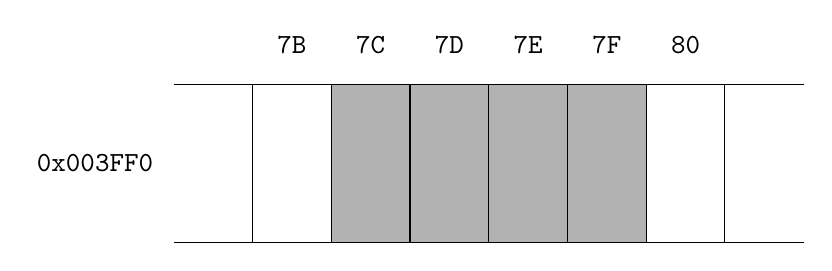
\begin{tikzpicture}
\def\arr{7B,7C,7D,7E,7F,80};
\draw (0,0) -- (8,0);
\draw (0,2) -- (8,2);
\edef\myleft{0}
\edef\myright{0}
\edef\mypos{0}
\foreach \item [count=\i] in \arr
{
	\ifthenelse{1<\i \AND \i<6}{%
		\fill[black!30!white] (\i,0) rectangle (\i+1,2);
	}{}
	\draw (\i,0) rectangle (\i+1,2);
	\node at (\i+0.5,2.5) {\texttt{\item}};
}
\node at (-1,1) {\texttt{0x003FF0}};
\end{tikzpicture}
\caption{變數 \lstinline!a! 實際的記憶體位置}
\label{program:struct:fig:int:address}
\end{figure}

\paragraph{}這個結果會因為不同機器、每次程式執行分配的記憶體而不同 (總之就是\textbf{不一定}啦!(╯°□°)╯︵ ╧╧),但概念是相同的。

\subsubsection{大字節序和小字節序}

\paragraph{}但是要怎麼知道變數 \lstinline!a! 實際怎麼儲存 \lstinline!16! 呢?很多人會以為像是圖 \ref{program:struct:fig:big:endian:16}:

\begin{figure}[h!]
\centering
\begin{tikzpicture}
\def\sz{3mm}
\def\mywd{7.5}
\def\myht{2.3}
\def\addr{7C,7D,7E,7F};
\def\arr{$00000000$,$00000000$,$00000000$,$00001000$};
\foreach \item [count=\i] in \arr
{
	\node[bit block] at (\i*\mywd*\sz,0) {\item};
}
\foreach \item [count=\i] in \addr
{
	\node at (\i*\mywd*\sz,.65) {\texttt{0x\item}};
}
\node at (0,0) {\texttt{0x003FF0}};
\end{tikzpicture}
\caption{大字節序儲存方法}
\label{program:struct:fig:big:endian:16}
\end{figure}

\paragraph{}但這個說法不完全對,圖 \ref{program:struct:fig:big:endian:16} 的儲存方法被稱為「\index{大字節序}{\textbf{大字節序}} (Big Endian)」,也就是 \lstinline!int! 的高位數會儲存在位址\textbf{比較小}的地方。
\paragraph{}另一種跟他相對的稱為「\index{小字節序}{\textbf{小字節序}} (Little Endian)」,也就是數字的高位數儲存在位址比較大的地方。用整數 \texttt{0x12345678} 來表示這兩種儲存方法,差異如圖 \ref{program:struct:fig:big:endian} 及 \ref{program:struct:fig:little:endian}:

\begin{figure}[h!]
\centering
\begin{subfigure}{0.4\textwidth}
  \centering
  \begin{tikzpicture}
\def\sz{3mm}
\def\mywd{4.5}
\def\myht{2.3}
\def\addr{7C,7D,7E,7F};
\def\arr{12,34,56,78};
\foreach \item [count=\i] in \arr
{
	\node[bit block] at (\i*\mywd*\sz,0) {\texttt{0x\item}};
}
\foreach \item [count=\i] in \addr
{
	\node at (\i*\mywd*\sz,.65) {\texttt{0x\item}};
}
  \end{tikzpicture}
  \caption{以大字節序儲存}
  \label{program:struct:fig:big:endian}
\end{subfigure}
~
\begin{subfigure}{0.4\textwidth}
  \centering
  \begin{tikzpicture}
\def\sz{3mm}
\def\mywd{4.5}
\def\myht{2.3}
\def\addr{7C,7D,7E,7F};
\def\arr{78,56,34,12};
\foreach \item [count=\i] in \arr
{
	\node[bit block] at (\i*\mywd*\sz,0) {\texttt{0x\item}};
}
\foreach \item [count=\i] in \addr
{
	\node at (\i*\mywd*\sz,.65) {\texttt{0x\item}};
}
  \end{tikzpicture}
  \caption{以小字節序儲存}
  \label{program:struct:fig:little:endian}
\end{subfigure}
\caption{\texttt{0x12345678} 不同儲存方法}
\label{program:struct:fig:big:little:endian}
\end{figure}

\paragraph{}之外,還有一類是「混合字節序 (Middle Endian)」,是大字節序和小字節序混用或者是其他的狀況,這裡不贅述。
\paragraph{}無論是大字節序還是小字節序,在程式當中都是表示「\texttt{0x12345678}」這個數字,這些儲存方法只是表示計算機\textbf{實際儲存資料}的差異,程式配置一塊記憶體用來儲存 \texttt{0x12345678},實際怎麼儲存在很多狀況下其實並不重要,但偶爾要做一些操作時,就會牽扯到這個概念。

\subsection{指標}

\paragraph{}\index{指標}{\textbf{指標}}是一個概念,他代表一個{\color{blue}\textbf{箭頭}}指向一塊記憶體。如圖 \ref{program:struct:fig:pointer}。

\begin{figure}[h!]
\centering
\begin{tikzpicture}
\def\arr{7B,7C,7D,7E,7F,80};
\draw (0,0) -- (8,0);
\draw (0,2) -- (8,2);
\edef\myleft{0}
\edef\myright{0}
\edef\mypos{0}
\foreach \item [count=\i] in \arr
{
	\draw (\i,0) rectangle (\i+1,2);
	\node at (\i+0.5,2.5) {\texttt{0x\item}};
}
\node at (-1,1) {\texttt{0x003FF0}};
\draw[line arrow] (2.5,4) -- (2.5,3);
\end{tikzpicture}
\caption{指標概念}
\label{program:struct:fig:pointer}
\end{figure}

\paragraph{}\texttt{C++} 是利用{\color{red}\textbf{儲存記憶體位址}}的方式實做指標,如何實現一個指標我們慢慢細說。

\subsubsection{宣告}

\paragraph{}首先,程式碼 \ref{program:struct:code:pointer:variable} 宣告一個\textbf{指標變數} \lstinline!ptr!。

\begin{code}[h!]
\centering
\begin{tabular}{c}
\begin{lstlisting}
int *ptr;
\end{lstlisting}
\end{tabular}
\caption{宣告指標變數 \lstinline!ptr!}
\label{program:struct:code:pointer:variable}
\end{code}

\paragraph{}宣告指標\textbf{變數}的規則,和之前宣告變數都是相同的原則:\textbf{變數名稱}和\textbf{用途},此時 \lstinline!ptr! 的資料型態為 \lstinline!int*!,代表這是一個指向 \lstinline!int! 的指標。因為資料型態是 \lstinline!int*!,所以也可用程式碼 \ref{program:struct:code:pointer:variable:another} 的方式來宣告。

\begin{code}[h!]
\centering
\begin{tabular}{c}
\begin{lstlisting}
int* ptr;
\end{lstlisting}
\end{tabular}
\caption{宣告指標變數 \lstinline!ptr!}
\label{program:struct:code:pointer:variable:another}
\end{code}

\paragraph{}值得注意的點是,當宣告多個指標變數時,不能寫成 \lstinline!int* ptr, ptr2!,在這個情形下,\texttt{C++} 會把 \lstinline!ptr2! 宣告成 \lstinline!int!,正確宣告多指標變數要像程式碼 \ref{program:struct:code:pointer:variable:multiple}。

\begin{code}[h!]
\centering
\begin{tabular}{c}
\begin{lstlisting}
int *ptr, *ptr2;
\end{lstlisting}
\end{tabular}
\caption{宣告多個指標變數}
\label{program:struct:code:pointer:variable:multiple}
\end{code}

\subsubsection{賦值}

\paragraph{}剛剛說過,指標的運作是讓指標變數儲存\textbf{位址},如果以之前變數 \lstinline!a! 的例子來講,我們知道變數 \lstinline!a! 的位址是 \texttt{0x003FF07C},若我們要把 \lstinline!ptr! 指向變數 \lstinline!a! 所在的記憶體,我們可以用先前講過的\textbf{取址運算子},得到 \lstinline!a! 的位址,如程式碼 \ref{program:struct:code:pointer:assignment}。

\begin{code}[h!]
\centering
\begin{tabular}{c}
\begin{lstlisting}
int a = 16;
int *ptr = &a;
\end{lstlisting}
\end{tabular}
\caption{指標的賦值}
\label{program:struct:code:pointer:assignment}
\end{code}

\paragraph{}程式碼 \ref{program:struct:code:pointer:assignment} 的實際狀況如圖 \ref{program:struct:fig:pointer:assignment}。

\begin{figure}[h!]
\centering
\begin{tikzpicture}
\def\myht{3};
\def\mywd{1};
\def\cont{0x003FF07C,16};
\def\addr{0x003FF080,0x003FF07C};
\def\name{\lstinline!ptr!,\lstinline!a!};
\foreach \item [count=\i] in \cont {
	\draw (5*\i,0) rectangle (5*\i+\myht,\mywd)%
		node[black,pos=.5] {\texttt{\item}};
	\ifthenelse{1<\i}{
		\draw[line arrow] (5*\i-5+\myht,0.5) -- (5*\i,0.5);
	}{}
}
\foreach \item [count=\i] in \addr {
	\node at (\myht/2+5*\i,-0.4) {\texttt{\item}};
}
\foreach \item [count=\i] in \name {
	\node at (\myht/2+5*\i,0.3+\mywd) {\item};
}
\end{tikzpicture}
\caption{程式碼 \ref{program:struct:code:pointer:assignment} 的狀況}
\label{program:struct:fig:pointer:assignment}
\end{figure}

\paragraph{}由圖 \ref{program:struct:fig:pointer:assignment} 可以看出以下幾個重點:
\begin{itemize}
\item 指標只是一個概念,實際上用變數來代表,既然 \texttt{C++} 的指標也是一個變數,那麼就需要另外配置記憶體。
\item \texttt{C++} 實做指標,就是{\color{blue}\textbf{儲存位址}}。
\end{itemize}

\subsubsection{取值運算子}

\paragraph{}指標最大的用處,就是可以知道{\color{red}\textbf{指向位址的值}},\texttt{C++} 中取得指向位址的值使用\index{取值運算子}{\textbf{取值運算子}} \lstinline!*!,以程式碼 \ref{program:struct:code:pointer:value} 為例。

\begin{code}[h!]
\centering
\begin{tabular}{c}
\begin{lstlisting}
int a = 16;
int b = 4;
int *ptr = &a;
cout << *ptr << endl;
ptr = &b;
cout << *ptr << endl;
\end{lstlisting}
\end{tabular}
\caption{取值運算子}
\label{program:struct:code:pointer:value}
\end{code}

\paragraph{}程式碼 \ref{program:struct:code:pointer:value} 中,第 4 行的 \lstinline!*! 是取值運算子 (這符號容易和指標宣告搞混),回傳指向記憶體的值,因此會印出「\lstinline!16!」。
\paragraph{}在第 5 行中,因為 \texttt{C++} 的指標也是一變數,因此會將 \lstinline!b! 的位址儲存在 \lstinline!ptr! 裡面,意義是指向變數 \lstinline!b!,因此第 6 行會印出 \lstinline!b! 的值,也就是「\lstinline!4!」。

\paragraph{}不同的資料型態,都有對應的指標型態,例如指向 \lstinline!int! 的指標型態為 \lstinline!int*!、指向 \lstinline!double! 的指標型態為 \lstinline!double*!,以此類推。以下情況由讀者做觀察,想想為什麼會有這些現象,有和預想中的不一樣嗎?
\begin{itemize}
\item \lstinline!sizeof(int*)! 和 \lstinline!sizeof(int)!
\item \lstinline!sizeof(long long*)! 和 \lstinline!sizeof(long long)!
\item \lstinline!sizeof(double*)! 和 \lstinline!sizeof(double)!
\end{itemize}

\paragraph{}此外,讀者可以觀察一下程式碼 \ref{program:struct:code:pointer:practice},這一章節主要是讓大家能夠了解指標的概念,並非以熟練指標為主:

\begin{code}[h!]
  \centering
  \begin{tabular}{c}
  \begin{lstlisting}
int a = 16;
int *ptr = &a;
cout << "Value of a = "   <<  a << endl;
cout << "Address of a = " << &a << endl;
cout << "Value of *ptr = "  << *ptr << endl;
cout << "Value of ptr = "   <<  ptr << endl;
cout << "Address of ptr = " << &ptr << endl;
  \end{lstlisting}
  \end{tabular}
  \caption{指標小練習}
  \label{program:struct:code:pointer:practice}
\end{code}

\paragraph{}除此之外,我們也可對指標所指的對象\textbf{進行運算},如程式碼 \ref{program:struct:code:pointer:operation}。

\begin{code}[h!]
\centering
\begin{tabular}{c}
\begin{lstlisting}
int a = 16;
int *ptr = &a;
(*ptr)++;
cout << a << endl;
\end{lstlisting}
\end{tabular}
\caption{指標操作}
\label{program:struct:code:pointer:operation}
\end{code}

\paragraph{}在程式碼 \ref{program:struct:code:pointer:operation} 中,第 4 行會印出「\lstinline!17!」,因為第 3 行的 \lstinline!*ptr! 是先對 \lstinline!ptr! 取值,得到變數 \lstinline!a! 的值,接著對 \lstinline!a! 做 \lstinline!++!。要注意的是我們是對「\lstinline!ptr! 所指的值做累加」,讀者可以比較 \lstinline!ptr++!、\lstinline!*ptr++! 與 \lstinline!(*ptr)++! 的不同。

\paragraph{}有了基本的指標概念之後,我們接下來看「指標的指標」,一個 \lstinline!int! 指標的型態為 \lstinline!int*!,如果是指向 \lstinline!int*! 的指標,則型態為 \lstinline!int**!,用法和普通的指標相似,程式碼 \ref{program:struct:code:pointer:of:pointer} 展示它的用法。

\begin{code}[h!]
\centering
\begin{tabular}{c}
\begin{lstlisting}
int a = 16;
int *ptr, **tmp;
ptr = &a;
tmp = &ptr;
cout << "a:" << endl;
cout << "Value of a = "    <<  a << endl;
cout << "Address of &a = " << &a << endl;
cout << "ptr:" << endl;
cout << "Value of ptr = "    <<  ptr << endl;
cout << "Value of *ptr = "   << *ptr << endl;
cout << "Address of &ptr = " << &ptr << endl;
cout << "tmp:" << endl;
cout << "Value of tmp = "    <<  tmp << endl;
cout << "Value of *tmp = "   << *tmp << endl;
cout << "Address of &tmp = " << &tmp << endl;
\end{lstlisting}
\end{tabular}
\caption{指標的指標}
\label{program:struct:code:pointer:of:pointer}
\end{code}

\paragraph{}讀者可以參考圖 \ref{program:struct:fig:pointer:of:pointer},第二行同時宣告 \lstinline!int*! 和 \lstinline!int**! 兩種指標,分別是變數 \lstinline!ptr! 和 \lstinline!tmp!,其中 \lstinline!ptr! 指向變數 \lstinline!a!,\lstinline!tmp! 指向變數 \lstinline!ptr!,其餘不贅述。

\begin{figure}[h!]
\centering
\begin{tikzpicture}
\def\myht{3};
\def\mywd{1};
\def\name{{"tmp","ptr","a"}};
\def\cont{{"0x003FF084","0x003FF080","0x003FF07C",16}};
\foreach \i in {0,...,2} {
	\pgfmathsetmacro{\addr}{\cont[\i]};
	\pgfmathsetmacro{\txt}{\cont[\i+1]};
	\pgfmathsetmacro{\tag}{\name[\i]};
	\draw (5*\i,0) rectangle (5*\i+\myht,\mywd)
		node[pos=.5] {\texttt{\txt}};
	\node at (5*\i+\myht/2,-0.4)      {\texttt{\addr}};
	\node at (5*\i+\myht/2,0.3+\mywd) {\texttt{\tag}};
}
\foreach \i in {0,...,1} {
	\draw[line arrow] (5*\i+\myht,0.5) -- (5*\i+5,0.5);
}
\end{tikzpicture}
\caption{程式碼 \ref{program:struct:code:pointer:of:pointer} 的狀況}
\label{program:struct:fig:pointer:of:pointer}
\end{figure}

\paragraph{}比較特別的是以下操作,如果程式碼 \ref{program:struct:code:pointer:of:pointer} 連續運用取址運算子和取值運算子,會有什麼結果呢?
\begin{itemize}
\item \lstinline!**tmp! 的值為何?
\item \lstinline!*&ptr! 和 \lstinline!&*ptr! 有什麼不同?
\item \lstinline!&&a! 可以運作嗎?
\end{itemize}

\subsubsection{資料型態}

\paragraph{}程式碼 \ref{program:struct:code:pointer:type} 展示了指標型態的用途,這個例子比較複雜,在第 2 行時,型態為 \lstinline!char*! 的指標 \lstinline!ptr!「刻意」去接 \lstinline!x! 的位址,但由於 \lstinline!x! 位址的型態為 \lstinline!int*!,因此得做型別轉換。

\begin{code}[h!]
\centering
\begin{tabular}{c}
\begin{lstlisting}
int x = 0x01020304;
char* ptr = (char*)&x;
cout << (int)*ptr << endl;
\end{lstlisting}
\end{tabular}
\caption{指標型態的用途}
\label{program:struct:code:pointer:type}
\end{code}

\paragraph{}接著第三行我們把 \lstinline!ptr! 指向的值轉換成 \lstinline!int! 輸出,會得到 \lstinline!0x01020304! 的十進位數字嗎?不會,否則就不會這樣問了。
\paragraph{}我們回頭來探討記憶體和資料型態的關係,前面有提到記憶體就好比是「\textbf{土地}」,土地可以規劃為住宅用、工業用土地等等。
\paragraph{}\index{宣告}{宣告}一個變數,相當於程式會配給變數一塊記憶體,但是這個記憶體的「\textbf{用途}」,就是看宣告時的資料型態,例如 \lstinline!int x! 的型態是 \lstinline!int!,因此程式才會知道要配給變數 \lstinline!x! 四個位元組。
\paragraph{}同樣的情況也發生在指標身上,指標也需要知道他指向的記憶體用途為何,才能依照該有的格式去存取。程式碼 \ref{program:struct:code:pointer:type} 第 2 行,當我們利用 \lstinline!char*! 指標去指向 \lstinline!x! 的位址,\lstinline!ptr! 實際上會把它所指向的記憶體當作 \lstinline!char! 來存取,如圖 \ref{program:struct:fig:pointer:type}。

\begin{figure}[h!]
\centering
\begin{tikzpicture}
\def\sz{3mm}
\def\mywd{4.5}
\def\myht{4.5}
\tikzset{selected bit block/.style={
	draw,
	rectangle,
	fill=black!40!white,
	minimum height=\myht*\sz,
	minimum width=\mywd*\sz
}}
\def\addr{X,X+1,X+2,X+3};
\node[selected bit block] at (\mywd*\sz,0) {};
\foreach \item [count=\i] in \addr
{
	\node at (\i*\mywd*\sz,.8*\myht*\sz) {\texttt{\item}};
	\node[bit block] at (\i*\mywd*\sz,0) {};
}
\node at (-.4*\sz,0) {變數 \lstinline!x!};
\end{tikzpicture}
\caption{實際上 \lstinline!ptr! 的有效範圍}
\label{program:struct:fig:pointer:type}
\end{figure}

\paragraph{}為了簡化描述,我們將變數 \lstinline!x! 第一個位元組的位址稱為 \texttt{X},依序為 \texttt{X+1}、\texttt{X+2}、\texttt{X+3}。當我們用 \lstinline!ptr! 指向位址 \lstinline!X! 時,因為 \lstinline!ptr! 會\textbf{認定}他指到的資料是 \lstinline!char!,因此輸出時只會輸出一個位元組的資料,也就是位址為 \lstinline!X! 所存的資料。
\paragraph{}然而最終答案會因為不同電腦而有差異,還記得大字節序和小字節序嗎?如果是大字節序的儲存方法,位址 \lstinline!X! 儲存的數字為 \texttt{0x01},而小字節序會儲存 \texttt{0x04}。

\subsubsection{空指標}

\paragraph{}在 \texttt{C++} 中,為了避免未初始化的指標指向未知記憶體,我們會用\index{空指標}{空指標}\textbf{常數} \lstinline!NULL! 來操作,嚴格來說,\lstinline!NULL! 不是空指標,而要經過型別轉換為指標型態後,也就是 \lstinline!(int*)NULL! 之類的操作,才會變為空指標。

\begin{code}[h!]
\centering
\begin{tabular}{c}
\begin{lstlisting}
#include <cstddef>

int* x = NULL;
int* y = (int*)NULL;
int* z = nullptr;
\end{lstlisting}
\end{tabular}
\caption{空指標用法}
\label{program:struct:code:pointer:null}
\end{code}

\paragraph{}程式碼 \ref{program:struct:code:pointer:null},示範了清空指標的方法。在 \texttt{C++11} 中,標頭檔 \index{標頭檔!cstddef}{\lstinline!<cstddef>!} 提供了空指標 \lstinline!nullptr! 可供使用。

\subsection{記憶體操作}

\paragraph{}這一段介紹 \texttt{C++} 除了指標之外,一些對記憶體常見的操作方法,以下兩個函式在 \index{標頭檔!cstring}{\lstinline!<cstring>!} 中:

\begin{code}[h!]
\centering
\begin{tabular}{c}
\begin{lstlisting}
void* memset(void* ptr, int value, size_t num);
void* memcpy(void* destination, const void* source, size_t num);
\end{lstlisting}
\end{tabular}
\caption{兩個常用的函式}
\label{program:struct:code:memory:function}
\end{code}

\paragraph{}這兩個函式的回傳值是 \index{void}{\lstinline!void*!},什麼意思呢?\lstinline!void! 有兩層意義:

\begin{itemize}
\item 當回傳型態為 \lstinline!void! 時,代表這個函式「{\color{red}\textbf{沒有回傳值}}」;
\item 當回傳型態為一個 \lstinline!void*! 指標型態時,這個指標會指向某一塊記憶體,此塊記憶體的用途是「無型態」,也就是\textbf{單純}當作記憶體來使用,不把他看做 \lstinline!int!、\lstinline!double! 等型態。
\end{itemize}

\subsubsection{\lstinline!memset! 函式}

\paragraph{}\lstinline!memset! 函式傳三個參數:\lstinline!ptr!、\lstinline!value! 和 \lstinline!num!,其中 \lstinline!ptr! 會指向一塊記憶體,\lstinline!memset! 函式的目的是將 \lstinline!ptr! 指向的記憶體中,把前 \lstinline!num! 個{\color{blue}\textbf{位元組}}的值改成 \lstinline!value!。

\begin{code}[h!]
\centering
\begin{tabular}{c}
\begin{lstlisting}
int x;
memset(&x, 1, sizeof(x));
cout << x << endl;
\end{lstlisting}
\end{tabular}
\caption{\lstinline!memset! 的基本用法}
\label{program:struct:code:memset:basic}
\end{code}

\paragraph{}舉例來說,假設我們有一個 \lstinline!int! 變數 \lstinline!x!,如程式碼 \ref{program:struct:code:memset:basic},猜猜變數 \lstinline!x! 會是多少呢?哈,答案並不是「\lstinline!1!」!
\paragraph{}剛剛提到,\lstinline!ptr! 只有單純指向記憶體,既然是視為記憶體。那它就是\textbf{一個位元組一個位元組}依序修改,因此程式碼 \ref{program:struct:code:memset:basic} 的結果會像圖 \ref{program:struct:fig:memset:basic}。

\begin{figure}[h!]
\centering
\begin{tikzpicture}
\def\sz{3mm}
\def\mywd{7.5}
\def\myht{2.3}
\foreach \i in {1,2,...,4}
{
	\node[bit block] at (\i*\mywd*\sz,0) {$0000000{\color{red}\textbf{1}}$};
}
\end{tikzpicture}
\caption{程式碼 \ref{program:struct:code:memset:basic} 得到的結果}
\label{program:struct:fig:memset:basic}
\end{figure}

\paragraph{}由此可知:
\begin{itemize}
\item 因為每次都是把每個位元組初始化,所以 \lstinline!value! 的值會介於 \lstinline!0! 到 \lstinline!255! 之間。常用的值有兩個:\lstinline!0! 和 \lstinline!-1! (\lstinline!255!),因為這兩個數字在二進位下代表全 \lstinline!0! 和全 \lstinline!1!,因此可以把數字都設為 \lstinline!0! 和 \lstinline!-1!,讀者不妨驗證一下。
\item 第三個參數是代表要初始化多少個位元組,往往我們都是初始化\textbf{所有}位元組,與其親自計算初始化的變數有多少位元組,不如取巧使用 \lstinline!sizeof! 運算子
\end{itemize}

\paragraph{}最後 \lstinline!memset! 函式會回傳修改資料後的 \lstinline!ptr! 指標。

\subsubsection{\lstinline!memcpy! 函式}

\paragraph{}這個函式與 \lstinline!memset! 類似,只是差在 \lstinline!memcpy! 就是把 \lstinline!source! 指標的資料,{\color{blue}\textbf{複製}}前 \lstinline!num! 個位元組到 \lstinline!destination! 指標所指的記憶體。如程式碼 \ref{program:struct:code:memcpy:basic} 約略敘述它的用法,之後會介紹比較廣泛的用途。

\begin{code}[h!]
\centering
\begin{tabular}{c}
\begin{lstlisting}
int x, y;
x = 5;
y = 2;
memcpy(&x, &y, sizeof(y));
cout << x << endl;
\end{lstlisting}
\end{tabular}
\caption{\lstinline!memcpy! 用法}
\label{program:struct:code:memcpy:basic}
\end{code}

\paragraph{}最後,\lstinline!memcpy! 會回傳 \lstinline!destination! 指標。

\section{程式控制}

\paragraph{}程式語言中,在語法上會設計一些用來方便表達我們思想的工具,這些工具經過幾十年的演變後,歸納出大部分程式語言會有的特性,以下介紹幾個 \lstinline!C++! 當中基本但重要的工具。

\subsection{程式區塊}

\paragraph{}\lstinline!C++! 中大括號被稱為\index{程式區塊}{程式區塊},用以包住多個程式敘述。試試看程式碼 \ref{program:struct:code:scope:example} 的兩個例子會發生什麼事?

\begin{code}[h!]
\centering
\begin{subcode}{.43\textwidth}
  \centering
  \begin{tabular}{c}
  \begin{lstlisting}
int main() {
  {
    int x = 2;
  }
  cout << x << endl;
}
  \end{lstlisting}
  \end{tabular}
  \caption{被大括號包住的 \lstinline!x!}
  \label{program:struct:code:scope:example:1}
\end{subcode}
~
\begin{subcode}{.43\textwidth}
  \centering
  \begin{tabular}{c}
  \begin{lstlisting}
int main() {
  int x = 2;
  {
    cout << x << endl;
  }
}
  \end{lstlisting}
  \end{tabular}
  \caption{另一個例子}
  \label{program:struct:code:scope:example:2}
\end{subcode}
\caption{程式區塊}
\label{program:struct:code:scope:example}
\end{code}

\paragraph{}\texttt{C++} 中的變數有\index{可視範圍}{\textbf{可視範圍 (Scope)}} 的觀念,通常變數會以{\color{blue}\textbf{函式、大括號}}做為區隔。例如程式碼 \ref{program:struct:code:scope:example:1} 中,變數 \lstinline!x! 被包含在大括號中,狀況如圖 \ref{program:struct:fig:scope:example:1}。

\begin{figure}[h!]
\centering
\begin{subfigure}{.35\textwidth}
  \centering
  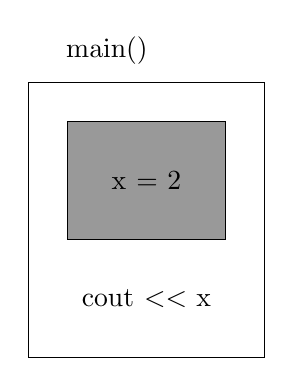
\begin{tikzpicture}
  \def\mywd{3};
  \def\myht{3.5};
  \draw (0,0) rectangle (\mywd,\myht);
  \filldraw[black!40!white,draw=black]%
	(.5,1.5) rectangle (\mywd-.5,\myht-.5)%
	node[black,pos=.5] {\lstinline!x = 2!};
  \node at (1,\myht+.4) {\lstinline!main()!};
  \node at (\mywd/2,.75) {\lstinline!cout << x!};
  \end{tikzpicture}
  \caption{\ref{program:struct:code:scope:example:1} 變數 \lstinline!x! 的可視範圍}
  \label{program:struct:fig:scope:example:1}
\end{subfigure}
~
\begin{subfigure}{.35\textwidth}
  \centering
  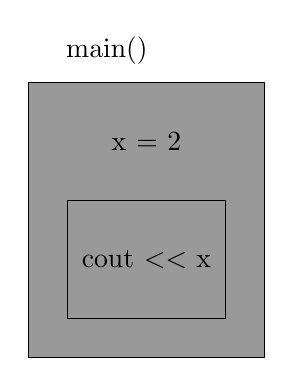
\begin{tikzpicture}
  \def\mywd{3};
  \def\myht{3.5};
  \filldraw[black!40!white,draw=black]%
	(0,0) rectangle (\mywd,\myht);
  \draw (.5,.5) rectangle (\mywd-.5,\myht-1.5)%
	node[pos=.5] {\lstinline!cout << x!};
  \node at (1,\myht+.4) {\lstinline!main()!};
  \node at (\mywd/2,\myht-.75) {\lstinline!x = 2!};
  \end{tikzpicture}
  \caption{\ref{program:struct:code:scope:example:2} 變數 \lstinline!x! 的可視範圍}
  \label{program:struct:fig:scope:example:2}
\end{subfigure}
\caption{程式碼 \ref{program:struct:code:scope:example} 的狀況}
\label{program:struct:fig:scope:example}
\end{figure}

\paragraph{}變數的可視範圍就像洋蔥一樣,外面一層的變數可以被裡面一層的變數看見,因此程式碼 \ref{program:struct:code:scope:example:1} 的 \lstinline!cout! 沒辦法看見包在大括號的變數 \lstinline!x!。

\paragraph{}程式碼 \ref{program:struct:code:scope:example:2} 展示另外一個例子,結果如圖 \ref{program:struct:fig:scope:example:2},雖然變數 \lstinline!x! 在外層,但裡面的 \lstinline!cout! 會一層一層往外找變數 \lstinline!x!,結果就是輸出 \lstinline!2!。

\paragraph{}詳細的可視範圍觀念留在之後說明。

\subsection{選擇結構}
\subsubsection{\lstinline!if! 結構}

\paragraph{}選擇結構在 \texttt{C++} 中就是 \lstinline!if!。\lstinline!if! 最簡單的語法如程式碼 \ref{program:struct:code:if:usage}。

\begin{code}[h!]
\centering
\begin{subcode}{.4\textwidth}
  \centering
  \begin{tabular}{c}
  \begin{lstlisting}
int a = 4;
if (a < 10)
  cout << a << endl;
  \end{lstlisting}
  \end{tabular}
  \caption{單行指令}
  \label{program:struct:code:if:usage:1}
\end{subcode}
~
\begin{subcode}{.4\textwidth}
  \centering
  \begin{tabular}{c}
  \begin{lstlisting}
int a = 4;
if (a < 10) {
  a += 5;
  cout << a << endl;
}
  \end{lstlisting}
  \end{tabular}
  \caption{程式區塊}
  \label{program:struct:code:if:usage:2}
\end{subcode}
\caption{\lstinline!if! 的用法}
\label{program:struct:code:if:usage}
\end{code}

\paragraph{}綜觀兩種情況,在 \lstinline!if! 後面的小括號放\textbf{邏輯運算式},只要邏輯運算式為 \lstinline!true!,就會執行後面的語句,若要執行多行語句,則要使用程式區塊用大括號括好。
\paragraph{}這個結構可以幫助設計一個條件開關,若 \lstinline!true! 執行某些程式;反之,若是 \lstinline!false! 則否。因此程式碼 \ref{program:struct:code:if:usage:1} 第 3 行,和程式碼 \ref{program:struct:code:if:usage:2} 第 3 行至第 5 行會被執行。

\subsubsection{\lstinline!if!\texttt{-}\lstinline!else! 結構}

\paragraph{}條件判斷更可進階為 \lstinline!if!\texttt{-}\lstinline!else! 結構,語法如程式碼 \ref{program:struct:code:if:else}。\lstinline!if!\texttt{-}\lstinline!else! 做的是:當邏輯運算式的結果為 \lstinline!true!,執行 \lstinline!if! 的區塊;如果是 \lstinline!false!,則執行 \lstinline!else! 區塊。

\begin{code}[h!]
\centering
\begin{tabular}{c}
\begin{lstlisting}
int a = 4;
if (a < 3)
  cout << "Yes!" << endl;
else
  cout << "QQ" << endl;
\end{lstlisting}
\end{tabular}
\caption{\lstinline!if!\texttt{-}\lstinline!else! 結構}
\label{program:struct:code:if:else}
\end{code}

\paragraph{}同樣地,\lstinline!else! 也可以改為程式區塊。當你要判斷的條件比較多時,\lstinline!if!\texttt{-}\lstinline!else! 可以連用,如程式碼 \ref{program:struct:code:if:else:if}。

\begin{code}[h!]
\centering
\begin{tabular}{c}
\begin{lstlisting}
int a = 4;
if (a < 3)
  cout << "Case 1" << endl;
else if (3 <= a && a < 6)
  cout << "Case 2" << endl;
else
  cout << "Case 3" << endl;
\end{lstlisting}
\end{tabular}
\caption{\lstinline!if! 和 \lstinline!else! 連用}
\label{program:struct:code:if:else:if}
\end{code}

\paragraph{}程式碼 \ref{program:struct:code:if:else:if} 中 \lstinline!if!\texttt{-}\lstinline!else! 可以一直接續下去,除此之外,類似的結構也有 \lstinline!switch! 等,這裡不贅述。

\subsubsection{懸置 \lstinline!else! 問題}

\paragraph{}將程式碼 \ref{program:struct:code:dangling:else:1} 拔掉大括號,變成程式碼 \ref{program:struct:code:dangling:else:2},會有什麼差別?

\begin{code}[h!]
\centering
\begin{subcode}{.5\textwidth}
  \centering
  \begin{tabular}{c}
  \begin{lstlisting}
if (0) {
  if (0) cout << "QQ" << endl;
}
else cout << "XD" << endl;
  \end{lstlisting}
  \end{tabular}
  \caption{危險的 \lstinline!else!}
  \label{program:struct:code:dangling:else:1}
\end{subcode}
~
\begin{subcode}{.45\textwidth}
  \centering
  \begin{tabular}{c}
  \begin{lstlisting}
if (0)
  if (0) cout << "QQ" << endl;
else cout << "XD" << endl;
  \end{lstlisting}
  \end{tabular}
  \caption{編譯器會不知道是哪一個 \lstinline!if! 的 \lstinline!else!}
  \label{program:struct:code:dangling:else:2}
\end{subcode}
\caption{懸置的 \lstinline!else!}
\label{program:struct:code:dangling:else}
\end{code}

\paragraph{}不僅僅是程式敘述以分號結尾,實際上編譯器也無法得知 \lstinline!else! 是和哪一個 \lstinline!if! 匹配,因此在沒括大括號的情況下,最後一個 \lstinline!else! 通常會匹配到最近的 \lstinline!if!,讀者可以驗證這兩段程式碼的不同。

\subsection{迴圈結構}

\subsubsection{簡介}

\paragraph{}\texttt{C++} 中常用的迴圈結構有三種:\lstinline!while!、\lstinline!do ... while! 和 \lstinline!for! 迴圈,原理都是反覆檢查一個判斷式,如果結果為 \lstinline!true! 則執行對應程式區塊;直到判斷式為 \lstinline!false!,則跳出迴圈結構。
\paragraph{}新手常見的錯誤是無法使判斷式變為 \lstinline!false! 導致無法跳出迴圈,或是寫出一個判斷式為 \lstinline!false! 的迴圈,使程式不會執行到迴圈內部。以下比較這些迴圈結構來說明。

\begin{code}[h!]
\centering
\begin{subcode}{.48\textwidth}
\centering
\begin{tabular}{c}
\begin{lstlisting}
for (int i = 0; i < 10; i++) {
  cout << i << endl;
}
\end{lstlisting}
\end{tabular}
\caption{\lstinline!for! 語法}
\end{subcode}
~
\begin{subcode}{.48\textwidth}
\centering
\begin{tabular}{c}
\begin{lstlisting}
{
  int i = 0;
  while (i < 10) {
    cout << i << endl;
    i++;
  }
}
\end{lstlisting}
\end{tabular}
\caption{對應的 \lstinline!while! 語法}
\end{subcode}
\caption{\lstinline!for! 和 \lstinline!while! 的對應關係}
\label{program:struct:code:loop:for:while}
\end{code}

\paragraph{}程式碼 \ref{program:struct:code:loop:for:while} 是 \lstinline!for! 和 \lstinline!while! 語法間的對應。從 \lstinline!while! 的寫法可以看到小括號間是判斷式,除非 \lstinline!i < 10! 為 \lstinline!false!,就會反覆執行程式區塊。在 \lstinline!while! 迴圈中最後一行,\lstinline!i++! 決定了是否能跳出迴圈,因為在每次執行完迴圈時,\lstinline!i! 值會遞增,直到不小於 \lstinline!10!,判斷式變為 \lstinline!false! 因而跳出迴圈。

\paragraph{}\lstinline!for! 迴圈與 \lstinline!while! 迴圈結構的對應中,要注意在 \lstinline!for! 迴圈中宣告變數,效力相當於一個區塊變數,離開 \lstinline!for! 迴圈後變數就會被回收。

\paragraph{}\lstinline!do ... while! 的特色是\textbf{後置判斷},在至少須執行一次迴圈的場合可以使用,基本用法如程式碼 \ref{program:struct:code:do:while}。

\begin{code}[h!]
\centering
\begin{tabular}{c}
\begin{lstlisting}
int i = 0;
do {
  cout << i << endl;
} while (i < 0);
\end{lstlisting}
\end{tabular}
\caption{\lstinline!if! 和 \lstinline!else! 連用}
\label{program:struct:code:do:while}
\end{code}

\subsubsection{應用:找極值}

\paragraph{}極值問題,通常是從 $n$ 個元素間求最大值和最小值。

\paragraph{}我們先從最簡單的狀況來考慮:兩個數字。給你兩個數字 $a$、$b$,找最大值就接用 \lstinline!if! 下去判斷,如程式碼 \ref{program:struct:code:max:if}。

\begin{code}[h!]
\centering
\begin{tabular}{c}
\begin{lstlisting}
if (a < b)
  cout << b << endl;
else
  cout << a << endl;
\end{lstlisting}
\end{tabular}
\caption{\lstinline!if! 求最大值}
\label{program:struct:code:max:if}
\end{code}

\paragraph{}內建函數的話,\index{標頭檔!iostream}{\lstinline!<iostream>!} 中有 \lstinline!max! 函數和 \lstinline!min! 函數,使用方法如程式碼 \ref{program:struct:code:max:max}。

\begin{code}[h!]
\centering
\begin{tabular}{c}
\begin{lstlisting}
cout << max(a, b) << endl;
\end{lstlisting}
\end{tabular}
\caption{\lstinline!max! 求最大值}
\label{program:struct:code:max:max}
\end{code}

\paragraph{}現在考慮原本的問題,$n$ 個數字下的極值,因為 \lstinline!max!、\lstinline!min! 等函數只能對兩個數字做比較,若是用 \lstinline!if! 去把所有可能做分類,如程式碼 \ref{program:struct:code:max:cases},除非是來不及寫正解的前提下,這類程式碼一來龐大、難以維護,一來如果出錯也不好 debug。

\begin{code}[h!]
\centering
\begin{tabular}{c}
\begin{lstlisting}
if (a < b < c)
  cout << c << endl;
else if (a < c < b)
  cout << b << endl;
else if (b < a < c)
  cout << c << endl;
else if (b < c < a)
  cout << a << endl;
else if (c < a < b)
  cout << b << endl;
else
  cout << a << endl;
\end{lstlisting}
\end{tabular}
\caption{\lstinline!if! 求 3 個數字最大值}
\label{program:struct:code:max:cases}
\end{code}

\paragraph{}如果我們善用迴圈和變數,迴圈可以走過所有數字,再利用一個變數 \lstinline!mx! 去儲存前 $i$ 個比較過後的最大值,迴圈開始前需要初始化這個變數,通常是第一個數字。

\paragraph{}程式碼 \ref{program:struct:code:max:for} 實作了這個想法,筆者在迴圈當中使用 \lstinline!if! 作為判斷,如果新的數字比之前比較過的最大值還要大,就可以替換成更大的數字,迴圈最後會使得 \lstinline!mx! 是 $n$ 個數字中的最大值。

\begin{code}[h!]
\centering
\begin{tabular}{c}
\begin{lstlisting}
int mx = a[0]; // 陣列 a 是 n 個數字
for (int i = 1; i < n; i++)
  if (mx < a[i])
    mx = a[i];
cout << mx << endl;
\end{lstlisting}
\end{tabular}
\caption{求 $n$ 個數字最大值}
\label{program:struct:code:max:for}
\end{code}


\paragraph{}如果沒辦法初始化為第一個數字時,那麼求最大值的初始值就讓他盡可能的小,使得往後讀到的第一個數字一定能取代他,求出來的最大值一定是在 $n$ 個數字中,例如:求極值的範圍是 \lstinline!int! 的範圍時,可令最大值 \lstinline!mx = -2147483648!,亦即 \lstinline!int! 中最小的數;如果求極值的範圍是正浮點數,則令最大值為隨便一個負數即可 \lstinline!mx = -1.0!。類似的道理,求最小值的時候,令初始值盡可能的大即可。

\subsubsection{應用:輸入測資}

\paragraph{}競賽中常見的輸入形式有三種:\textbf{EOF 版}、\textbf{0 尾版}、\textbf{n 行版},其他少部分的形式在了解以下基本的輸入法和一些 IO 應用後都不難構造,因此要好好理解。

\paragraph{0 尾版}典型的 0 尾版是題目要求:「輸入以 $n = 0$ 結束。」我們可以這樣做:

\begin{code}[h!]
\centering
\begin{tabular}{c}
\begin{lstlisting}
while (cin >> n, n) {
  cout << n << endl;
}
\end{lstlisting}
\end{tabular}
\caption{0 尾版}
\label{program:struct:code:loop:input:0:ending}
\end{code}

\paragraph{}程式碼 \ref{program:struct:code:loop:input:0:ending} 利用逗號運算子和比較運算子的簡化,當輸入為零時,逗號右側的 \lstinline!n! 會判定為 \lstinline!false! 而跳出迴圈。

\paragraph{}類似 0 尾版的輸入可能是以特定的數字做為結束 (常見的是 \lstinline!-1!),有時會以多個數字是否全零、是否為特定字串作為結尾,讀者可以自行練習。

\paragraph{n 行版}典型 n 行版的輸入為:「第一行有一個整數 $n$,代表接下來的測試資料筆數。」因此在設計上,我們要優先讀入此整數,再處理各組測試資料。一種寫法如程式碼 \ref{program:struct:code:loop:input:n:lines}:

\begin{code}[h!]
\centering
\begin{tabular}{c}
\begin{lstlisting}
for (cin >> n; n; n--) {
  cout << n << endl;
}
\end{lstlisting}
\end{tabular}
\caption{$n$ 行版}
\label{program:struct:code:loop:input:n:lines}
\end{code}

\paragraph{}程式碼 \ref{program:struct:code:loop:input:n:lines} 也是利用邏輯運算子簡化,每次執行完迴圈 \lstinline!n! 就會遞減,直到第 $n$ 次做完後,回頭檢查 \lstinline!n! 值為零而退出迴圈。
\paragraph{}另外一種常見形式是題目要求形如「\lstinline!"Case #:"!」的輸出,這時就要使用一個變數去計算目前執行到的資料筆數,如程式碼 \ref{program:struct:code:loop:input:n:lines:case}。

\begin{code}[h!]
\centering
\begin{tabular}{c}
\begin{lstlisting}
for (cin >> n, cnt = 1; cnt <= n; cnt++) {
  cout << "Case " << cnt << ":" << endl;
}
\end{lstlisting}
\end{tabular}
\caption{$n$ 行版的另一種形式}
\label{program:struct:code:loop:input:n:lines:case}
\end{code}

\paragraph{\texttt{EOF} 版}當題目敘述提到:「以 \texttt{EOF} 結束」,或是沒有特別提到結束的方式,且在輸入中不是前面兩種形式結尾通常都是 \texttt{EOF} 版。
\paragraph{}\texttt{EOF} 是 end-of-file 的簡寫,意思是輸入到檔案結尾,沒有測試資料就可結束。當 \lstinline!cin! 讀取到檔案結尾時,會「知道」讀取到檔案結尾,因此設計上可寫為程式碼 \ref{program:struct:code:loop:input:eof}。

\begin{code}[h!]
\centering
\begin{tabular}{c}
\begin{lstlisting}
while (cin >> n) {
  cout << n << endl;
}
\end{lstlisting}
\end{tabular}
\caption{\texttt{EOF} 版}
\label{program:struct:code:loop:input:eof}
\end{code}

\paragraph{}在測試執行當中,如果要用鍵盤輸入檔案結尾,依據作業系統的不同而有差異,大致上是 \texttt{Ctrl+Z} 或是 \texttt{Ctrl+D}。

\subsection{陣列}

\subsubsection{簡介}

\paragraph{}\textbf{{\color{red}注意!}\lstinline!C++! 陣列 index 從 0 開始!}

\subsubsection{指標運算}

\begin{code}[h!]
\centering
\begin{tabular}{c}
\begin{lstlisting}
int a[5] = { 1, 4, 9, 16, 25 };
int *ptr = &a[1];
cout << ptr << endl;
cout << *ptr << endl;
cout << ptr + 1 << endl;
cout << *(ptr + 1) << endl;
\end{lstlisting}
\end{tabular}
\caption{指標加法}
\label{program:struct:code:array:pointer:addition}
\end{code}

\paragraph{}試試看下面語句,解釋輸出結果:

\begin{itemize}
\item \lstinline!*(&a[0] + 1)!
\item \lstinline!&a[1] - &a[0]!
\item \lstinline!(char *)&a[1] - (char *)&a[0]!
\item \lstinline!(long long *)&a[1] - (long long *)&a[0]!
\item \lstinline!(void *)&a[1] - (void *)&a[0]!
\end{itemize}

\subsubsection{陣列指標}

\paragraph{}事實上,陣列本身是一種指標,例如程式碼 \ref{program:struct:code:array:pointer},會印出陣列本身的位址,此種指標型態為 \lstinline!int(*)[5]!,可以把 \lstinline!int[5]! 看成是一種資料型態,代表五個 \lstinline!int!,\lstinline!int(*)[5]! 是指向 \lstinline!int[5]! 的指標,\lstinline![5]! 清楚表示指向的記憶體有五個 \lstinline!int! 的長度,而與此對應的 \lstinline!int*! 則沒有標示有多少個 \lstinline!int! 的長度。

\begin{code}[h!]
\centering
\begin{tabular}{c}
\begin{lstlisting}
int a[5] = { 1, 4, 9, 16, 25 };
int *p = a; // int* 指向陣列 a
cout << a << endl;
cout << a + 1 << endl;  // a[1] 的位址
cout << &a + 1 << endl; // 指標運算跳過整個陣列
\end{lstlisting}
\end{tabular}
\caption{陣列指標}
\label{program:struct:code:array:pointer}
\end{code}

\paragraph{}配合上面的指標運算,陣列的\index{運算子!下標運算子}{下標運算子} \lstinline!a[x]! 實際上就等同於 \lstinline!*(a + x)!。程式碼 \ref{program:struct:code:array:pointer}。

\subsection{函數}

\paragraph{}將陣列傳入函數,事實上是傳入陣列指標。

\subsubsection{傳值呼叫}

\begin{code}[h!]
\centering
\begin{tabular}{c}
\begin{lstlisting}
void c8763(int x) {
  x++;
  return;
}
int main() {
  int a = 0;
  c8763(a);
  cout << a << endl; // 0
}
\end{lstlisting}
\end{tabular}
\caption{傳值呼叫}
\label{program:struct:code:function:pass:value}
\end{code}

\subsubsection{傳址呼叫}

\paragraph{}\texttt{C} 語言一開始的設計是用指標。

\begin{code}[h!]
\centering
\begin{tabular}{c}
\begin{lstlisting}
void c8763(int *x) {
  (*x)++;
  return;
}
int main() {
  int a = 0;
  c8763(&a);
  cout << a << endl; // 1
}
\end{lstlisting}
\end{tabular}
\caption{傳址呼叫}
\label{program:struct:code:function:pass:address}
\end{code}

\subsubsection{傳參考呼叫}

\paragraph{}\texttt{C++} 中,有另外一種傳參考呼叫,相當於是「\textbf{別名}」。

\begin{code}[h!]
\centering
\begin{tabular}{c}
\begin{lstlisting}
void c8763(int &x) { // 參考
  x++;
  return;
}
int main() {
  int a = 0;
  c8763(a);
  cout << a << endl; // 1
}
\end{lstlisting}
\end{tabular}
\caption{傳參考呼叫}
\label{program:struct:code:function:pass:reference}
\end{code}

\subsubsection{函數多載}

\subsubsection{函數指標}

\paragraph{}函數也有\index{指標!函數指標}{指標},例如對於傳兩個 \lstinline!int! 參數、回傳值為 \lstinline!int! 的函數而言,其指標型態為 \lstinline!int(*)(int,int)!,在此以程式碼 \ref{program:struct:code:function:pointer} 簡單介紹,不贅述。

\begin{code}[h!]
\centering
\begin{tabular}{c}
\begin{lstlisting}
int f(int a, int b) { return a + b; }
int g(int a, int b) { return a - b; }
int h(int (*func)(int, int), int a, int b) {
  return func(a, b);
}
int main() {
  cout << h(f, 1, 2) << endl; // 3
  cout << h(g, 2, 1) << endl; // 1
}
\end{lstlisting}
\end{tabular}
\caption{函數指標}
\label{program:struct:code:function:pointer}
\end{code}

\subsection{\texttt{C++} 物件導向}

\paragraph{}這一節主要提供一些 \texttt{C++} 物件導向的方法,來增加競賽寫程式的速度及方便性,並不會提到太多物件導向的觀念,想要知道更多有關這方面的讀者可以在網路上搜尋。

\subsubsection{物件與類別}

\paragraph{}在物件導向的世界裡,我們把所有東西都視為一個又一個的\index{物件導向!物件}{\color{red}\textbf{物件 (Object)}},這些物件都有各自的\textbf{內部狀態}--也就是物件本身會儲存各式各樣的資料,而這些物件之間會相互影響,進而改變內部的狀態,這就是物件導向的核心概念。
\paragraph{}物件有其\textbf{生命週期},當物件被產生時,物件會呼叫\index{物件導向!建構子}{\textbf{建構子 (Constructor)}} 初始化,當物件的生命結束要被消滅時,物件會呼叫\index{物件導向!解構子}{\textbf{解構子 (Destructor)}},在物件內的函式可以表達物件的行為模式,以及如何影響其他物件,此時這些函式稱為\index{物件導向!方法}{\color{blue}\textbf{方法 (Method)}}。
\paragraph{}物件導向中的物件,是由\index{物件導向!類別}{\color{red}\textbf{類別 (Class)}} 所產生,若類別 A 產生了一個物件 B,我們稱 B 是 A 的一個\index{物件導向!實例}{\textbf{實例 (Instance)}}。類別好比是一張製作物件的{\color{blue}\textbf{藍圖}},裡面記載創造的物件需要能夠儲存什麼資料,提供什麼方法等等。
\paragraph{}當程式開始執行時,程式會先創造一塊記憶體來存放藍圖。創造實例時,創造出的物件會依據類別所包含的變數、方法來創造。在 \texttt{C++} 中,\lstinline!struct! 和 \lstinline!class! 都被當成類別的一種,當我們要寫一個複數的類別時,可以寫如程式碼 \ref{program:struct:code:object:class}。

\begin{code}[h!]
\centering
\begin{subcode}{.4\textwidth}
  \centering
  \begin{tabular}{c}
  \begin{lstlisting}
struct Complex {
  double real, imag;
};
  \end{lstlisting}
  \end{tabular}
  \caption{\texttt{Complex} 結構}
  \label{program:struct:code:object:class:1}
\end{subcode}
~
\begin{subcode}{.4\textwidth}
  \centering
  \begin{tabular}{c}
  \begin{lstlisting}
class Complex {
public:
  double real, imag;
};
  \end{lstlisting}
  \end{tabular}
  \caption{\texttt{Complex} 類別}
  \label{program:struct:code:object:class:2}
\end{subcode}
\caption{結構和類別的對應}
\label{program:struct:code:object:class}
\end{code}

\paragraph{}要創造一個實例的話,其實就是\textbf{宣告變數} \lstinline!Complex c;!。

\subsubsection{建構子與解構子}

\paragraph{}上一節提到,物件被創造時會呼叫\index{物件導向!建構子}{\textbf{建構子}},結束時會呼叫解構子,在此節我們把注意力放在建構子上。
\paragraph{}通常變數宣告時,計算機並不會幫我們初始化變數,而變數的內容是\textbf{未知數},因此要避免使用未經初始化的變數。在物件導向的世界中,創造一個物件時會呼叫建構子--它可以看做是類別的一種方法,一個很特殊的方法。
\paragraph{}例如,我們想讓每個複數一開始都能被歸零,一種直觀的寫法如程式碼 \ref{program:struct:code:object:init}。

\begin{code}[h!]
\centering
\begin{tabular}{c}
\begin{lstlisting}
Complex c;
c.real = c.imag = 0.0;
\end{lstlisting}
\end{tabular}
\caption{初始化 \lstinline!Complex! 物件}
\label{program:struct:code:object:init}
\end{code}

\paragraph{}同樣功能如果要用建構子實作的話,一來每次宣告變數時會自動呼叫建構子初始化,二來在程式風格上同樣都是寫於類別內,比較不容易出現漏網之魚。

\begin{code}[h!]
\centering
\begin{tabular}{c}
\begin{lstlisting}
struct Complex {
  double real, imag;
  Complex() {
    real = imag = 0.0;
  }
};
\end{lstlisting}
\end{tabular}
\caption{\lstinline!Complex! 建構子}
\label{program:struct:code:object:constructor}
\end{code}

\paragraph{}建構子特別之處在於,
\begin{itemize}
\item 建構子不需要寫回傳值
\item 建構子名稱必為類別名稱,因此 \lstinline!Complex()! 即為 \lstinline!Complex! 類別的建構子
\end{itemize}

\paragraph{}此外,建構子也可以多載,如果想要初始化成特定數字,我們可以多寫一個建構子,如程式碼 \ref{program:struct:code:object:constructor:overload}。

\begin{code}[h!]
\centering
\begin{tabular}{c}
\begin{lstlisting}
struct Complex {
  double real, imag;
  Complex() {
    real = imag = 0.0;
  }
  Complex(double r, double i) {
    real = r;
    imag = i;
  }
};

Complex c1, c2(4.0,5.0);
\end{lstlisting}
\end{tabular}
\caption{\lstinline!Complex! 建構子多載}
\label{program:struct:code:object:constructor:overload}
\end{code}

\paragraph{}程式碼 \ref{program:struct:code:object:constructor:overload} 會將 \lstinline!c1! 的實部虛部初始化為 \lstinline!0!,而 \lstinline!c2! 會呼叫另外一個建構子,將實部初始化為 \lstinline!4.0!,而虛部為 \lstinline!5.0!。

\subsubsection{運算子多載}

\paragraph{}假設現在有兩個 \lstinline!Complex a,b!,我們要把這兩個複數相加,可以寫作程式碼 \ref{program:struct:code:object:operator:function}。

\begin{code}[h!]
\centering
\begin{tabular}{c}
\begin{lstlisting}
Complex compAdd(const Complex &left, const Complex &right) {
  return Complex(left.real + right.real, left.imag + right.imag);
}

Complex result = compAdd(a, b);
\end{lstlisting}
\end{tabular}
\caption{\lstinline!Complex! 相加}
\label{program:struct:code:object:operator:function}
\end{code}

\paragraph{}程式碼 \ref{program:struct:code:object:operator:function} 第 1 行中,\lstinline!const! 代表變數在此不會被改值,可以避免掉誤改的狀況。第 2 行呼叫建構子 \ref{program:struct:code:object:constructor:overload},創造一個新的 \lstinline!Complex! 物件並賦值。這種方法跟以往我們習慣處理這類問題時大不相同,如果不用建構子的話我們通常要先宣告一個複數,再把值放進去,如程式碼 \ref{program:struct:code:object:operator:naive}。

\begin{code}[h!]
\centering
\begin{tabular}{c}
\begin{lstlisting}
Complex compAdd(const Complex &left, const Complex &right) {
  Complex c;
  c.real = left.real + right.real;
  c.imag = left.imag + right.imag;
  return c;
}
\end{lstlisting}
\end{tabular}
\caption{\lstinline!Complex! 相加}
\label{program:struct:code:object:operator:naive}
\end{code}

\paragraph{}此外,原先的函式也可以放入 \lstinline!struct! 中,成為 \lstinline!struct! 的\index{物件導向!成員函式}{\textbf{成員函式 (Member Function)}}--也就是 \lstinline!Complex! 的一個方法。成員函式和 \lstinline!real!、\lstinline!imag! 等\index{物件導向!成員資料}{成員資料 (Member Data)} 的用法相同,使用\index{運算子!成員運算子}{「\lstinline!.!」運算子}來存取:

\begin{code}[h!]
\centering
\begin{tabular}{c}
\begin{lstlisting}
struct Complex {
  double real, imag;
  Complex() {
    real = imag = 0.0;
  }
  Complex(double r, double i) {
    real = r;
    imag = i;
  }
  Complex compAdd(Complex right) {
    return Complex(real + right.real, imag + right.imag);
  }
};

Complex res = a.compAdd(b);
\end{lstlisting}
\end{tabular}
\caption{\lstinline!Complex! 相加}
\label{program:struct:code:object:operator:member}
\end{code}

\paragraph{}程式碼 \ref{program:struct:code:object:operator:member} 可發現複數 \lstinline!a! 呼叫了 \lstinline!compAdd! 函數,並傳入複數 \lstinline!b!。在 \lstinline!compAdd! 中,因為此方法是 \lstinline!a! 的成員,因此可以直接使用 \lstinline!a! 的 \lstinline!real!、\lstinline!imag!。
\paragraph{}若要寫得更自然,像是 \lstinline!int! 做四則運算 \lstinline!a + b! 的寫法時,我們就要用到\index{運算子多載}{\color{red}\textbf{運算子多載 (Operator Overloading)}}。在 \texttt{C++} 中,運算子被當作成員函式一般,因此 \lstinline!a + b! 可視為

\begin{code}[h!]
\centering
\begin{tabular}{c}
\begin{lstlisting}
a.operator+(b);
\end{lstlisting}
\end{tabular}
\caption{運算子多載}
\label{program:struct:code:object:operator:add}
\end{code}

\paragraph{}程式碼 \ref{program:struct:code:object:operator:add} 的 \lstinline!operator+! 是函式名稱,代表加法運算。既然「加法」可被當作一種成員函式,因此也可以對 \lstinline!Complex! 類別多載「加法」,如程式碼 \ref{program:struct:code:object:operator:overload}。

\begin{code}[h!]
\centering
\begin{tabular}{c}
\begin{lstlisting}
struct Complex {
  double real, imag;
  Complex() {
    real = imag = 0.0;
  }
  Complex(double r, double i) {
    real = r;
    imag = i;
  }
  Complex operator+ (Complex right) {
    return Complex(real + right.real, imag + right.imag);
  }
};

Complex result = a + b;
\end{lstlisting}
\end{tabular}
\caption{運算子多載}
\label{program:struct:code:object:operator:overload}
\end{code}

\paragraph{}若要寫得更精準的話,我們知加法運算會把 \lstinline!a!、\lstinline!b! 兩者相加,但 \lstinline!a!、\lstinline!b! 本身值不變,這時就可以使用 \lstinline!const! 修飾,如程式碼 \ref{program:struct:code:object:operator:overload:const},其中後面的 \lstinline!const! 代表呼叫 \lstinline!operator+! 本身物件不會被修改,回傳值亦為一個新的 \lstinline!Complex! 物件。

\begin{code}[h!]
\centering
\begin{tabular}{c}
\begin{lstlisting}
Complex operator+ (const Complex &right) const {
  return Complex(real + right.real, imag + right.imag);
}
\end{lstlisting}
\end{tabular}
\caption{運算子多載}
\label{program:struct:code:object:operator:overload:const}
\end{code}

\paragraph{}其他運算子大多可以多載,在此不贅述。

\subsubsection{類別與物件}

\paragraph{}本節一開始有提到物件和類別之間的關係,依據種類,我們可以把類別內記載的資料分為以下四類:
\begin{itemize}
\item 實例屬性
\item 實例方法
\item 類別屬性
\item 類別方法
\end{itemize}

\paragraph{}實例屬性和方法即是物件所擁有的屬性和方法,例如 \lstinline!Complex! 類別中,每個實例擁有不一樣的 \lstinline!real!、\lstinline!imag! 等。

\begin{code}[h!]
\centering
\begin{tabular}{c}
\begin{lstlisting}
struct Circle {
  double r;
  Circle() {}
  Circle(double c) { r = c; }
  static double PI;
};

double Circle::PI = 3.14;

int main() {
  cout << Circle::PI << endl;
}
\end{lstlisting}
\end{tabular}
\caption{類別屬性}
\label{program:struct:code:object:static:attr}
\end{code}

\paragraph{}類別屬性和方法可以看做是整個類別所\textbf{共有}的,也就是在同個類別下所有物件,看到的類別屬性值都會是相同的,以程式碼 \ref{program:struct:code:object:static:attr} 為例,我們要建立 \lstinline!Circle! 類別,其中 \lstinline!Circle! 擁有一個實例屬性 \lstinline!r!,代表圓形的半徑。
\paragraph{}在 \lstinline!Circle! 類別中有一個類別屬性 \lstinline!PI!,以一個浮點數代表圓周率,一般來說圓周率是一個通用值,因此可以設為類別屬性,亦即往後創造的 \lstinline!Circle! 物件,所見的圓周率皆是相同的。
\paragraph{}設定一個屬性為類別屬性是在類別中用 \lstinline!static! 修飾,要{\color{red}\textbf{注意}}的是,類別屬性在類別內只能宣告,賦值需要在類別外賦值,可以參考程式碼 \ref{program:struct:code:object:static:attr} 第 8 行。若要使用類別屬性,需要使用\index{運算子!範圍解析運算子}{範圍解析運算子「\lstinline!::!」},使用方法如程式碼 \ref{program:struct:code:object:static:attr} 第 11 行。

\begin{code}[h!]
\centering
\begin{tabular}{c}
\begin{lstlisting}
struct Circle {
  double r;
  Circle() {}
  Circle(double c) { r = c; }
  static double PI;
  static double area(const Circle &c) {
    return c.r * c.r * PI;
  }
};

double Circle::PI = 3.14;

int main() {
  Circle c(1);
  cout << Circle::area(c) << endl;
}
\end{lstlisting}
\end{tabular}
\caption{類別方法}
\label{program:struct:code:object:static:method}
\end{code}

\paragraph{}類別方法用法也和類別屬性類似,程式碼 \ref{program:struct:code:object:static:method} 展示類別方法 \lstinline!Circle::area!。

\subsubsection{命名空間}

\paragraph{}\index{物件導向!命名空間}{\color{blue}\textbf{命名空間 (Namespace)}} 可以看做是管理程式碼的一種方法,在競賽之外往往會使用外部的標頭檔、第三方程式碼等,這些程式碼在變數、類別命名上會有同名的可能,為了避免同名導致編譯錯誤,我們會將程式碼裝入一個命名空間內 (類似一個很大的類別)。
\paragraph{}最直接的例子就是命名空間 \lstinline!std!,在第一章我們提到程式的基本架構中有一行:

\begin{code}[h!]
\centering
\begin{tabular}{c}
\begin{lstlisting}
using namespace std;
\end{lstlisting}
\end{tabular}
\caption{預設 \lstinline!std! 命名空間}
\label{program:struct:code:namespace:std}
\end{code}

\paragraph{}程式碼 \ref{program:struct:code:namespace:std} 代表我們在沒有指定使用何命名空間的東西時,預設就是使用 \lstinline!std! 內的物件、函數等,如 \lstinline!std::cin!、\lstinline!std::cout!、\lstinline!std::sort! 等等。

\section{程式技巧}
\subsection{函式化與結構化}

\paragraph{}當輸入、解題、輸出較為複雜時,可以做以下的函式化:

\begin{code}[h!]
\centering
\begin{tabular}{c}
\begin{lstlisting}
while ( input() ) {
  sol();
  output();
}
\end{lstlisting}
\end{tabular}
\caption{函式化程式}
\label{program:struct:code:input:function}
\end{code}

\paragraph{}函式化雖然理論上會慢一些,但是可以換來以下好處,使得我們可以方便除錯:
\begin{itemize}
\item 易於閱讀。程式碼 \ref{program:struct:code:input:function} 可以清楚看出此程式區塊大致上在處理多筆輸入,針對每筆輸入解出對應解答並輸出。
\item 易於撰寫。當你將解題所需大部分的工作都規劃成函式,那麼只要將每個函式個功能寫出來後,只要想法正確、沒有 bug,基本上都能一次 AC。
\end{itemize}
\paragraph{}程式碼 \ref{program:struct:code:input:function:example:main} 是一個函式化的範例程式碼片段,除去 \lstinline!#define! 等用法之外,雖然我們不知道題目是什麼,但可以清楚看出 \lstinline!input()! 可以是每次讀完測資之後,讓 \lstinline!sol()! 函數處理並回傳答案。

\begin{code}[h!]
\centering
\begin{tabular}{c}
\begin{lstlisting}
#define MAX 1010
int n, a[MAX];

int main() {
  while (input()) printf("%d\n", sol());
}
\end{lstlisting}
\end{tabular}
\caption{函式化範例 (\lstinline!main! 部分)}
\label{program:struct:code:input:function:example:main}
\end{code}

\paragraph{}接著看 \lstinline!input()! 部分,程式碼 \ref{program:struct:code:input:function:example:input} 可以看出是 0 尾版的輸入,只是 \lstinline!input()! 是放在 \lstinline!while! 的判斷條件內,因此無論是 0 尾、n 行、EOF 等,只要讀到一筆測資就回傳 \lstinline!true!,反之則回傳 \lstinline!false!。

\begin{code}[h!]
\centering
\begin{tabular}{c}
\begin{lstlisting}
int input() {
  for (n = 0; scanf("%d", &a[n]), a[n]; n++)
    if (n) a[n - 1] -= a[n];
  return n;
}
\end{lstlisting}
\end{tabular}
\caption{函式化範例 (\lstinline!input! 部分)}
\label{program:struct:code:input:function:example:input}
\end{code}

\paragraph{}最後,看看 \lstinline!sol()!,可以一眼看出這個題目使用了求最大公因數 \lstinline!gcd! (除非寫程式的人亂取名字)、\lstinline!sol! 用到 \lstinline!gcd! 求出答案。

\begin{code}[h!]
\centering
\begin{tabular}{c}
\begin{lstlisting}
int gcd(int a, int b) {
  if (b) return gcd(b, a % b);
    return a;
}
int sol() {
  int i, g = abs(a[0]);
  for (i = 1; i < n - 1; i++)
    g = gcd(g, abs(a[i]));
  return g;
}
\end{lstlisting}
\end{tabular}
\caption{函式化範例 (\lstinline!sol! 部分)}
\label{program:struct:code:input:function:example:sol}
\end{code}

\paragraph{}函式化容易辨識出哪個部分負責什麼樣的工作,因此就會比較好除錯。函式化的缺點就是程式碼容易變長、程式可能會較慢等等,但事實上寫程式的速度主要是思考、除錯的時間,除非在寫秒殺題,否則都是思考的時間居多,因此程式碼變長沒什麼關係,重點在於讓你除錯的時間變快,容易理解的程式碼也會加快除錯的速度。

\subsection{\lstinline!\#define!}

\subsection{標準模板函式庫}
\subsubsection{模板}

\paragraph{}之前有學過函式多載,例如我們自己要寫一個取最小值的函數 \lstinline!myMin!,我們可以自己寫一個判斷 \lstinline!int! 最小值的函數:

\begin{code}[h!]
\centering
\begin{tabular}{c}
\begin{lstlisting}
int myMin(int x, int y) {
  if (x < y)
    return x;
  return y;
}
\end{lstlisting}
\end{tabular}
\caption{\lstinline!myMin! 函數}
\label{program:struct:code:template:mymin:int}
\end{code}

\paragraph{}但是可以取最小值的資料型態不只有 \lstinline!int!,也可能是 \lstinline!double!、\lstinline!long long!、\lstinline!short!、...等等,於是我們就需要寫出很多版本的最小值函數:

\begin{code}[h!]
\centering
\begin{subcode}{\textwidth}
  \centering
  \begin{tabular}{c}
  \begin{lstlisting}
double myMin(double x, double y) {
  if (x < y)
    return x;
  return y;
}
  \end{lstlisting}
  \end{tabular}
  \caption{\lstinline!double! 版本}
  \label{program:struct:code:template:mymin:double}
\end{subcode}
~
\begin{subcode}{\textwidth}
  \centering
  \begin{tabular}{c}
  \begin{lstlisting}
long long myMin(long long x, long long y) {
  if (x < y)
    return x;
  return y;
}
  \end{lstlisting}
  \end{tabular}
  \caption{\lstinline!long long! 版本}
  \label{program:struct:code:template:mymin:long:long}
\end{subcode}
\caption{其他 \lstinline!myMin! 函數}
\label{program:struct:code:template:mymin}
\end{code}

\paragraph{}可以看出程式碼 \ref{program:struct:code:template:mymin} 中,除了宣告之外其餘部分與 \ref{program:struct:code:template:mymin:int} 完全相同,雖然我們可以利用函式多載完成所有最小值,但我們寫出了重複的程式,為此,\texttt{C++} 提供的模板功能,模板相當於是一個「程式碼」的{\color{red}\textbf{範本}},當需要什麼類型的程式碼時,再自動「抄寫出」對應的一份程式碼出來。

\begin{code}[h!]
\centering
\begin{tabular}{c}
\begin{lstlisting}
template<class T>
T myMin(T x, T y) {
  if (x < y)
    return x;
  return y;
}
int main() {
  cout << myMin(1, 2) << endl;
  cout << myMin(2.5, 3.5) << endl;
}
\end{lstlisting}
\end{tabular}
\caption{使用 \lstinline!template! 的 \lstinline!myMin! 函數}
\label{program:struct:code:template:mymin:template}
\end{code}

\paragraph{}程式碼 \ref{program:struct:code:template:mymin:template} 使用了模板功能,會在函數前宣告 \lstinline!template<class T>!,此時 \lstinline!T! 可以看做是資料型態的變數,程式會在{\color{red}\textbf{編譯時期}}檢查需要哪些種類的 \lstinline!myMin! 函數,例如程式碼第 8 行,在編譯時期會產生函數 \lstinline!int myMin(int, int)!,而在第 9 行,編譯器會知道需要 \lstinline!double! 版本的 \lstinline!myMin!,而產生 \lstinline!double myMin(double, double)!。
\paragraph{}此外,模板的參數也可以有很多個,程式碼 \ref{program:struct:code:template:class:multi} 會用到兩種資料型態,一個命名為 \lstinline!__Tx!、另一命名為 \lstinline!__Ty!。

\begin{code}[h!]
\centering
\begin{tabular}{c}
\begin{lstlisting}
template<class __Tx, class __Ty>
\end{lstlisting}
\end{tabular}
\caption{使用兩種 \lstinline!class! 的模板}
\label{program:struct:code:template:class:multi}
\end{code}

\paragraph{}模板也可套用在類別上,假設我們要儲存二維平面上的座標,類別 \lstinline!Point! 可以寫作程式碼 \ref{program:struct:code:template:point:class}。

\begin{code}[h!]
\centering
\begin{tabular}{c}
\begin{lstlisting}
struct Point {
  int x, y;
};
\end{lstlisting}
\end{tabular}
\caption{\lstinline!Point! 類別}
\label{program:struct:code:template:point:class}
\end{code}

\paragraph{}若要儲存浮點數的二維座標的話,可以考慮利用 \lstinline!template!,如程式碼 \ref{program:struct:code:template:point:template} 第 5、6 行,分別是儲存 \lstinline!int! 和 \lstinline!double! 座標的 \lstinline!Point! 類別。\texttt{C++} 的 STL 中很多是以 \lstinline!template! 實作。

\begin{code}[h!]
\centering
\begin{tabular}{c}
\begin{lstlisting}
template<class T>
struct Point {
  T x, y;
};
Point<int> p1;
Point<double> p2;
\end{lstlisting}
\end{tabular}
\caption{\lstinline!Point! 類別}
\label{program:struct:code:template:point:template}
\end{code}

\paragraph{}競賽中,可以對模板進行遞迴,因為模板會在編譯時期生成程式,而編譯時間不會計算在執行時間,因此有一些建表策略可以考慮在模板當中實行。這個方法被稱為\textbf{模板後設編程 (Template metaprogramming)}。
\paragraph{}程式碼 \ref{program:struct:code:template:fibo} 用\index{費氏數列}{費氏數列}作為例子,前四行定義了費式數列的遞迴式,。

\begin{code}[h!]
\centering
\begin{tabular}{c}
\begin{lstlisting}
template<int n>
struct fib {
  static const int val = fib<n - 1>::val + fib<n - 2>::val;
};
template<> // fib[1] = 1;
struct fib<1> {
  static const int val = 1;
};
template<> // fib[0] = 0;
struct fib<0> {
  static const int val = 0;
};

int main() {
  cout << fib<10>::val << endl;
  int x = 10;
  cout << fib<x>::val << endl; // error
}
\end{lstlisting}
\end{tabular}
\caption{費氏數列遞迴}
\label{program:struct:code:template:fibo}
\end{code}

\paragraph{}最簡單使用模板的方法。

\begin{code}[h!]
\centering
\begin{tabular}{c}
\begin{lstlisting}
template<int n>
struct fib {
  enum { val = fib<n - 1>::val + fib<n - 2>::val };
  static void init(vector<int> &v) {
    fib<n - 1>::init(v);
    v.push_back( val );
  }
};

template<>
struct fib<0> {
  enum { val = 0 };
  static void init(vector<int> &v) {
    v.push_back( val );
  }
};

template<>
struct fib<1> {
  enum { val = 1 };
  static void init(vector<int> &v) {
    fib<0>::init(v);
    v.push_back( val );
  }
};
\end{lstlisting}
\end{tabular}
\caption{把費氏數列裝進 \lstinline!vector! 中}
\label{program:struct:code:template:fibo:vector}
\end{code}

\paragraph{}要注意的是,程式碼 \ref{program:struct:code:template:fibo:vector} \lstinline!fib<1>! 中,靜態方法 \lstinline!init! 會呼叫 \lstinline!fib<0>::init!,若 \lstinline!fib<0>! 在此之前未定義會出現編譯錯誤。

\begin{code}[h!]
\centering
\begin{tabular}{c}
\begin{lstlisting}
vector<int> f;
fib<40>::init(f);
int x = 40;
for (int i = 0; i < x; i++)
  cout << f[i] << endl;
\end{lstlisting}
\end{tabular}
\end{code}

\subsubsection{迭代器}

\subsubsection{計算頻率}

\subsection{\lstinline!<algorithm>! 函式庫}

\subsection{其他注意事項}

\subsubsection{有關測試資料}

\paragraph{範例測資無法代表一切}有些人會有疑問:「阿我範例測資過了,為啥還是不會 AC?」所謂的範例測資,就是「\textbf{範例}」測資,只是提供幾個當作參考,可能故意漏掉一些重要的資訊讓你 WA 掉,或是誤導你的想法可是範例測資會讓你正確等等陰險手段。

\paragraph{AC 未必是正解}有種東西叫做「假解」,就是存在非正解但卻可以 AC 的程式碼,例如說某個問題的正解要 DP,但有人爆搜卻過了;明明有個測資會讓你 WA 掉可是卻 AC 了 ... 以此類推。
\paragraph{}有時是測資量不夠,沒有能夠讓假解不能過的特殊測資,或者是寫了正解,少部分的程式碼寫錯但卻 AC (這個最嚴重 ... 寫到類似題往往會認為自己是正確的),因此有時候 AC 了,只是僥倖,不能代表你程式碼完全正確。

\paragraph{邊界測資}很多人會忽略所謂「\textbf{邊界測資}」,就是題目輸入範圍內最極限的測資,忽略邊界測資往往會造成 WA 或 RE。
\paragraph{}例如,計算費氏數列第 $n$ 項 ($0\leq{n}\leq{100}$),那麼第 $0$ 項、第 $100$ 項便是值得注意的範圍;問你 $a^b$ 的值,那麼你要注意 $0^b$、$a^0$、$0^0$ 等等這些異常莫名其妙的測資 (除非題目保證說沒有,不然都得考慮)。

\paragraph{小結}綜觀以上情形,平常最好是多思考更多測資去檢查自己的想法,很多時候不管是 AC 還是 WA 都僅僅是參考。
\paragraph{}想測資往往是一件滿困難的事,但多想可以加強思考力,除錯時最關鍵常常是邊界測資。有時候邊界測資會是一個奇形怪狀的東西,只要符合題目敘述,就有可能是讀者思考中遺漏掉的邊界測資。

\subsubsection{記憶體與程式風格}

\paragraph{使用記憶體不見得要精準}在解題比賽時,記憶體是不是用得恰當,只要題目能 AC、寫起來寫得順就行!實作上只要開「{\color{blue}\textbf{夠大}}」的陣列就好了,例如:需要長度為 100 的陣列,可以開長度為 110 的陣列,原因是我們不必花太多心思去決定邊界到底是 100 還是 101 這回事上 (別忘了在比賽,有些細節可以不必太要求)。
\paragraph{}有些題目設計上會\textbf{要求}記憶體的使用,這類題目主要是在於使用不同的資料結構而有差異,通常 110 和 100 的陣列這點浪費記憶體不足以影響結果 (機率低)。例如,某個資料結構需要 $100010\times{100010}$,在大多數的機器上是無法宣告這麼大的二微陣列,但替換成另一個資料結構與演算法,可能讓使用的記憶體減少至 $3\times{100010}$。

\paragraph{小心遞迴}遞迴時會使用到系統堆疊,這時就要注意演算法是會因為遞迴過深造成 RE。

\subsubsection{除錯相關}

\paragraph{}常常上傳後,得到的結果是 WA,此時最著名的第一個反應是:「不可能會寫錯呀?一定是 judge 有問題 ... bla bla。」等到抓到錯誤才恍然大悟:「哦~原來只是這樣 ... bla bla。」
\paragraph{}\textbf{除錯 (debug)} 也是寫程式重要的一個環節,一個程式如果不想除錯,就不要寫出有 bug 的程式,但常常事與願違。由於程式是自己寫出來的,面對自己的程式碼,最大的困難點在於會認為「自己沒有寫錯」。最好的解法就是要記得每次找到錯誤時,要稍微記得自己在哪裡出錯,或是要注意大家常常出錯的地方。
\paragraph{}例如在學 \texttt{C++} 初期,常常會把邏輯運算式的「相等」少寫一個 \lstinline!=!,如程式碼 \ref{program:struct:code:debug:if}。

\begin{code}[h!]
\centering
\begin{tabular}{c}
\begin{lstlisting}
if (a = 5) ...
\end{lstlisting}
\end{tabular}
\caption{比較運算子誤寫}
\label{program:struct:code:debug:if}
\end{code}

\paragraph{}或是陣列的使用上超出範圍 (程式碼 \ref{program:struct:code:debug:array})。

\begin{code}[h!]
\centering
\begin{tabular}{c}
\begin{lstlisting}
int a[100];
for (i = 1; i <= 100; i++)
cin >> a[i];
\end{lstlisting}
\end{tabular}
\caption{比較運算子誤寫}
\label{program:struct:code:debug:array}
\end{code}

\paragraph{}其他常見的 bug 如下:

\begin{itemize}
\item 打{\color{red}\textbf{錯字}},包括 \lstinline!==! 打成 \lstinline!=!,打錯數字、符號等等
\item 應注意的事項{\color{blue}\textbf{未注意}},例如:輸出格式不對,陣列大小不對,忘記初始化,忘記 \lstinline!return! 等等
\item 操作上的錯誤,例如:傳錯程式碼,傳錯題目,{\color{blue}\textbf{忘記存檔}},{\color{red}\textbf{除錯訊息忘記拿掉}}等
\end{itemize}

\subsubsection{喇賽}

\paragraph{}當你沒辦法想出正解時,{\color{red}\textbf{喇賽}}是必要的途徑。不要以為隨便亂寫不重要,其實到最後不管是初學者還是高手,總會遇到不知道怎麼解的題目 (或是刻意出正解很難、但是喇賽就會過的題目),這時候就是比較誰喇賽功力的強弱了!
\paragraph{}通常喇賽可以是很\textbf{多個演算法}混在一起;\textbf{爆搜、剪枝}再加一些東西;或者根本\textbf{亂寫}。很多技巧都可以應用在喇賽領域,有些人光靠喇賽 AC 但別人寫正解卻會 TLE (這有發生過),因此喇賽是比賽的「終極」--很多時候在分測資點的比賽中也還是會撈到一些分數,但只要我們能夠將喇賽的技巧練得純熟,或許可能很快就不知道 WA 為何物了。
\paragraph{}快速上手喇賽技巧,就是遇到每一題都可以嘗試亂寫看看,那麼當你每一題都 AC 的時候就是你出師的時候了。

\section{程式執行}
\subsection{執行時期配置}

\paragraph{}前面提到程式需要放到記憶體中執行,實際上一支程式在記憶體中會有五個主要的區塊,每個區塊會放置特定的資料,程式架構和配置會因作業系統不同而有差異。

\begin{figure}[h!]
\centering
\begin{tikzpicture}
\def\myln{12};
\def\mywd{2};
\def\cont{{"TEXT","DATA","BSS","HEAP","","STACK"}};
\def\arr{{0,2,3.5,4.5,6,\myln-2,\myln}};
\foreach \i in {0,...,5} {
	\pgfmathsetmacro{\left}{\arr[\i]}
	\pgfmathsetmacro{\right}{\arr[\i+1]}
	\pgfmathsetmacro{\txt}{\cont[\i]}
	\draw (\left,0) rectangle (\right,\mywd)
		node[pos=.5] {\txt};
}
\pgfmathsetmacro{\left}{\arr[4]};
\pgfmathsetmacro{\right}{\arr[5]};
\def\myarrowln{1};
\draw[line arrow] (\left,\mywd/2) -- (\left+\myarrowln,\mywd/2);
\draw[line arrow] (\right,\mywd/2) -- (\right-\myarrowln,\mywd/2);
\node at (-1,\mywd/2) {程式};
\end{tikzpicture}
\caption{程式在記憶體執行的架構}
\label{program:struct:fig:program}
\end{figure}

\begin{itemize}
\item TEXT 區塊:編譯過後的二進位程式碼
\item DATA 區塊:有初始化的全域變數、靜態變數等
\item BSS 區塊:未初始化的全域變數、靜態變數等
\item HEAP 區塊:動態配置的變數等,使用一種稱為\index{堆積}{\textbf{堆積 (Heap)}} 的資料結構
\item STACK 區塊:函數呼叫、區域變數等,使用稱為\index{堆疊}{\textbf{堆疊 (Stack)}} 的資料結構
\end{itemize}

\paragraph{}這些區塊的概念清楚有助於除錯,有興趣的讀者可以自行 google。

\subsubsection{動態配置記憶體}

\begin{code}[h!]
\centering
\begin{tabular}{c}
\begin{lstlisting}
int *a = new int[10];
delete a;
\end{lstlisting}
\end{tabular}
\end{code}

\subsubsection{變數可視範圍}

\subsection{程式語言}

\subsubsection{直敘式語言}
\subsubsection{物件導向語言}
\subsubsection{機器語言與組合語言}

\subsection{程式編譯}

\ifx \allfiles \undefined

\printindex

\clearpage
\end{CJK}
\end{document}

\fi